\documentclass[12pt]{article}

\usepackage{amsmath}
\usepackage{amssymb}

%opening

\begin{document}

\begin{center}
\huge{Mathematics for Computing}\\
\LARGE{Functions}
\end{center}
\tableofcontents
\newpage
%------------------------------------------------------------------------%
\section{Sets of Numbers}

\begin{itemize}
\item $\mathbb{Z}$ Set of all integers
\item $\mathbb{Q}$ Set of all rational numbers
\item $\mathbb{R}$ Set of all real numbers
\end{itemize}


\begin{itemize}
\item $\mathbb{Z}^{+}$ Set of all positive integers
\item $\mathbb{Z}^{-}$ Set of all negative integers
\item $\mathbb{R}^{+}$ Set of all positive real numbers
\item $\mathbb{R}^{-}$ Set of all negative real numbers
\end{itemize}
% Session 4 - Functions

%------------------------------------------------------------------------%
\section{Arrow Diagrams}

\begin{itemize}

\item Domain
\item Co-Domain
\item Range
\end{itemize}
\[  f(x) : \mbox{Domain} \rightarrow \mbox{Co-Domain} \]
\[  f(x) : \mathbb{R} \rightarrow \mathbb{R} \]
%----------------------------------------------------------- %
\newpage
\subsection*{Polynomial Functions (4.1.5)}

\begin{itemize}
\item[Constants] $(P_0)$
\item[Linear Functions] $(P_1)$
\item[Quadratic Functions] $(P_2)$
\item[Cubic Functions] $(P_3)$
\end{itemize}


\subsection*{Equality of Functions (4.1.6)}
\[f(x) = g(x) \]

%------------------------------------------------------------------------%
\section{Special Mathematical Functions}
\subsection{Mathematical Operators}
\begin{itemize}
\item The Square Root function
\item The Floor and Ceiling functions
\item The Absolute Value functions
\end{itemize}


\begin{itemize}
\item Root Functions
\item Absolute Value Function
\item Floor Function
\item Ceiling Function
\end{itemize}
{
\large
\begin{eqnarray}
\lfloor 3.14 \rfloor =& 3 \\
\lceil -4.5 \rceil =& -5 \\
| -4 | =&  4
\end{eqnarray}
}
For this course, only positive numbers have square roots. The square roots are positive numbers. (This statement is not strictly true. The square root of a negative number is called a complex number. However this is not part of the course).

Negative numbers can have cube roots

{
\[ -27 = -3 \times -3 \times -3 \qquad \]
\LARGE
\[ \sqrt[3]{-27} = -3 \]
}
%-------------------------------------------------------------------------%

\newpage
\section{Exponential and Logarithms}
\subsection*{Laws of Logarithms}

\begin{itemize}
\item Law 1 : Multiplcation of Logarithms
\[ Log(a) \times Log(b) = Log(a+b) \]
\item Law 2 : Division of Logarithms
\[ \frac{Log(a)}{Log(b)} = Log(a-b) \]
\item Law 3 : Powers of Logarithms
\[ Log(a^b) = b \times Log(a) \]
\end{itemize}



%------------------------------------------------------%
\subsection{Exercise} 
$h(x): \mathbb{R} \rightarrow \mathbb{R}$ 
$g(x): \mathbb{R} \rightarrow \mathbb{R}$

\[f(x) = sqrt(x)\]
\[g(x) = \sqrt{3}{x+2}\]
\[h(x) = 2^x\]

\begin{itemize}
\item Is the function $h(x)$ an \textit{onto} function?
\item determine the inverse function of $h(x)$ and $g(x)$
\item Simplify the following function.
\[ j(x) = \mbox{log}_4(h(6x))\]
\end{itemize}
%--------------------------------------------%
\subsection{Onto Functions}
Definition: If every element in the co-domain of the function has an ancestor, the function is said to be "onto".
An onto function has the property that the domain is equal to the co-domain.


\textbf{Example 4.26 Page 53}

%--------------------------------------------%
\subsection*{Exponential and Logarithms}

\textbf{Rules}\\
Expontials : Rules 4.18 Page 58 \\
Logarithms : Rules 4.23 Page 61 \\

\[ log_a(a) = 1 \]
\[ log_a(b^c) = c \times log_a(b) \]

\begin{itemize}
\item $log_2(128) = 7$
\item $log_2(1/4) = -2$
\item $log_2(2) = 1$
\end{itemize}

\[ log_a(b) = \frac{log_x(b)}{log_x(a)} \]

%------------------------------------------------------%
\subsection{Logarithms} 
 - Laws of Logarithms
 - Change of Base
  
 \[ \mbox{Log}_b(x) = a \] \[b^a = x \]
 \[ \mbox{Log}_2(8) = 3 \] \[2^3 = 8 \]

 \[ \mbox{Log}_b(x) \times \mbox{Log}_b(y) =  \mbox{Log}_b(x+y) \]
 \[ \mbox{Log}_b(x^y) =  y \times \mbox{Log}_b(x) \]

 \[ \mbox{Log}_y(x)  =  \frac{ \mbox{Log}_b(x) }{ \mbox{Log}_b(y) } \]
%------------------------------------------------------%
\subsection{Exponents}
 - Rules of Exponents

\[ (a^b)^c = a^{b \times c}\]

\[ 64^{2/3} =  (4^3)^{2/3} = 4^{3\times2/3} = 4^2 = 16 \]


\[ (a^b) \times (a^c) = a^{b+c}\]
\[ (3^2) \times (3^3) = 3^{2+3} = 3^5  =243 \]

%------------------------------------------------------%
\textbf{Exercises}
\begin{itemize}
\item[(a)] 
Complete the following table for the functions 
\begin{itemize}
\item[i)] $g(x) = \mbox{log}_3x$,
\item[ii)] $h(x) =\sqrt[3]{x}$.
\end{itemize} 
\begin{center}

\begin{tabular}{|c||c|c|c|c|c|c|}
\hline $x$ &  \phantom{p}1\phantom{p}&  &  &  & 81 &  \\ 
\hline \phantom{p} $g(x)$ \phantom{p}&  & \phantom{p}1\phantom{p} & \phantom{p}2\phantom{p} &  &  &  \phantom{p}5\phantom{p} \\ 
\hline \phantom{p}$h(x)$ \phantom{p}&  &  &  &  3.00 & \phantom{p}\phantom{p}\phantom{p}  &  \\ 
\hline 
\end{tabular} 
\end{center}

Express your answers to 2 decimal places only.

\newpage
%------------------------------------------------------------------------%
\section{\textit{One-to-One} Functions and \textit{Onto} Functions}

\subsection{Invertible Functions}
\begin{itemize}
 \item One-to-One Function
 \item Onto Function
\end{itemize}

Onto Functions : Range and Co-Domain are equivalent

\subsection{Inverting a Function}

\begin{itemize}
\item[$\bullet$] You are given $f(x)$ in terms of $x$
\item[$\bullet$] Re-arrange the equation so that $x$ is given in terms of $f(x)$
\item[$\bullet$] Replace $x$ with $f^{-1}(x)$ and $f(x)$ with $x$
\end{itemize}

\subsubsection{Example}
\begin{itemize}
\item[$\bullet$]Determine the inverse function of $f(x)$. Re-arrange the equation so that $x$ is given in terms of $f(x)$
\[  f(x): \mathbb{R} \rightarrow \mathbb{R}  \mbox{   } f(x)  = \sqrt{x+1} \]
\item[$\bullet$] Square both sides of the equation.
\[[f(x)]^2 = x+1 \]
\item[$\bullet$] Subtract 1 from both sides of the equation. We have the equation written in terms of x.
\[f(x)^2-1 = x \]
\item[$\bullet$] Replace $x$ with $f^{-1}(x)$ and $f(x)$ with $x$
\[x^2-1 = f^{-1}(x) \]
\item[$\bullet$] 
 Re-arrange equation and specify domain and co-domain.
\[ f(x): \mathbb{R} \rightarrow \mathbb{R}  \mbox{   }  f^{-1}(x) = x^2-1  \]
\end{itemize}
% \[ f(x)  = \sqrt{x+1} \]
% \[f(x)^2 = x+1 \]
% \[f(x)^2-1 = x \]
% \[x^2-1 = f^{-1}(x) \]
\newpage
\section{Big O-Notation}

%------------------------------------------------------------------------%
% Section 4 Functions
% http://doc.gold.ac.uk/~maa01km/solutions/tut4sol.pdf

\item[(b)] Let $S$ be the set of all 4 bit binary strings. 

The function $f : S \rightarrow \mathbb{Z}$
is defined by the rule:
\[f(x) = \mbox{the number of zeros in x}\]
for each binary string $x \in S$.\\
Find:
\begin{enumerate}
\item the number of elements in the domain
\item $f(1000)$
\item the set of pre-images of 1
\item the range of $f$.
\end{enumerate}
\item[(c)]
\end{itemize}
\newpage
\begin{itemize}
\item[4.a] $ \lfloor x - y \rfloor = \lfloor x \rfloor - \lfloor y \rfloor$
\item[4.b]
\item[4.c]
\end{itemize}
\newpage
%------------------------------------------------------------------------%
\section{Section 4 Functions}

\subsection{Invertible Functions}
A function is invertible if it fulfils two criteria
\begin{itemize}
\item The function is \textbf{\textit{onto}},
\item The function is \textbf{\textit{one-to-one}}.
\end{itemize}

State the conditions to be satisfied by a function
$f : X \leftarrow Y$ for it to have an inverse function
$f^{-1} : Y \leftarrow X$.
%---------------------------------------------------------%

$\lceil \frac{x^2+1}{4} \rceil$
where $f : A \rightarrow \textbf{Z}$
\begin{itemize}
\item[(i)] Find $f(4)$ and the ancestors of 3.
\item[(ii)] Find the range of $f$.
\item[(iii)] Is f invertible? Justify your answer
\end{itemize}

Given $f : \textbf{R} \rightarrow \textbf{R}$ where f(x) =3x-1,define fully
the inverse of the function f ,i.e.$f^{-1}$. 
State the value of $f^{-1}(2)$
%---------------------------------------------------------%
\subsection{Precision Functions}

\begin{itemize}
\item Absolute Value Function $| x |$
\item Ceiling Function $\lceil x \rceil$
\item Floor Function  $\lfloor x \rfloor $
\end{itemize}
%\[ \lfloorx\rfloor\]

\noindent \textbf{Question1.2}: State the range and domain of the following function
\[ F(x) = \lfloor x-1 \rfloor \]
%---------------------------------------------------------%
\subsection{Powers}

\[  2^ 4 = 2 \times 2 \times 2 \times 2 = 16 \]

\[  5^ 3 = 5 \times 5 \times 5 =125 \]

\subsubsection{Special Cases}

Anything to the power of zero is always 1

\[  X^ 0 = 1 \mbox{ for all values of X} \]

Sometimes the power is a negative number.

\[  X^{-Y} = { 1 \over X^Y}  \]

Example 
\[  2^{-3} = { 1 \over 2^3} = { 1 \over 8}  \]



%---------------------------------------------------------%
\subsection{Exponentials Functions}

\[ e^a \times e^b = e^{a+b}\]

\[ (e^a )^b = e^{ab}\]
%---------------------------------------------------------%
\subsection{Logarithmic Functions}

\subsubsection{Laws for Logarithms}
The following laws are very useful for working with logarithms.
\begin{enumerate}
\item $\mbox{log}_b(X)$ + $\mbox{log}_b(Y)$ = $\mbox{log}_b(X\times Y)$
\item $\mbox{log}_b(X)$ - $\mbox{log}_b(Y)$ = $\mbox{log}_b(X / Y)$
\item $\mbox{log}_b(X^Y)$= $Y \mbox{log}_b(X)$
\end{enumerate}

\noindent \textbf{Question1.3} Compute the Logarithm of the following
\begin{itemize}
\item $\mbox{log}_2(8)$
\item $\mbox{log}_2(\sqrt{128})$
\item $\mbox{log}_2(64)$
\item $\mbox{log}_5(125)$ +   $\mbox{log}_3(729)$
\item $\mbox{log}_2(64/4)$
\end{itemize}

%----------------------------------------------------------------%

\begin{itemize}
\item $a^x = y$  $log_a(y) = x$

\item $e^x = y$  $ln(y)=x$

\item $log_a(x\times y) = log_a(x) + log_a(y)$

\item $log_a(\frac{x}{y}) = log_a(x) - log_a(y)$

\item $log_a(\frac{1}{x}) = - log_a(x)$

\item $log_a(a) = 1$

\item $log_a(1) = 0$
\end{itemize}


\begin{itemize}
\item $\lceil x\rceil$

\item $\lfloor x\rfloor$
\end{itemize}

\begin{tabular}{|c|c|c|c|}
\hline Sample value x & Floor $\lfloor x\rfloor$ & Ceiling  $\lceil x\rceil$ & Fractional part $ \{ x \} $\\
12/5 = 2.4 &	2	&3&	2/5 = 0.4\\
2.7&	2&	3	&0.7\\
-2.7&	-3&	-2	&0.3\\
-2&	-2&	-2	&0\\
\hline 
\end{tabular} 


\section*{Set Theory}

\begin{itemize}
	\item[1.1] Introduction  
	\item[1.2] Sets  
	\item[1.3] Sub-sets  
	\item[1.4] The order of sets: finite and infinite sets .
	\item[1.5] Union and intersection of sets  
	\item[1.6] Differences and complements  
	\item[1.7] Venn diagrams  
	\item[1.8] Logic analysis
\end{itemize}  
%-----------------------------------------------------%
\newpage
\subsection*{Union and intersection of sets}

\begin{itemize}
	\item The \textbf{union} of two sets A and B is a set containing all the elements in
	either A or B (or both)
	i.e. 
	\[A \cup B = {x / x \in A \mbox{ or } x \in B}.\]
	\item The \textbf{intersection} of two sets A and B is a set containing all the elements
	that are both in A and B
	i.e. 
	\[A \cap B = {x / x \in A \mbox{ and }x \in B}\].
	
	\item If sets A and B have no elements in common, i.e. $A \cap B = \emptyset$,then A and B
	are termed \textbf{disjoint sets}.
\end{itemize}
\newpage
\subsection*{Subsets}

\begin{itemize}
	\item Proper Subsets
\end{itemize}
\subsection*{The Power Set}

\newpage
\subsection*{Venn Diagrams}
%\begin{figure}
%\centering
%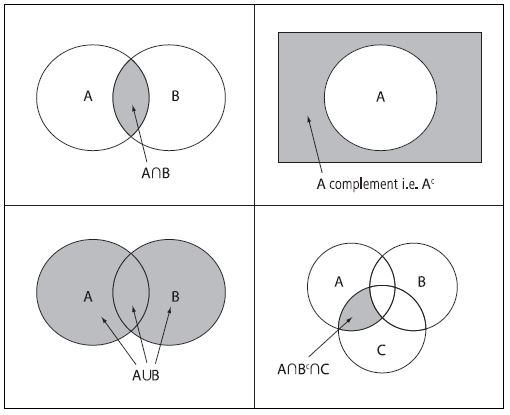
\includegraphics[width=0.7\linewidth]{venndiagram}
%
%\end{figure}
\[ \mbox{IMAGE}\]
\end{document}
Both oneone and onto
one one only
neither one ontoone or 
Arrow Diagram
onto functions (4:2:2)
Invertible Functions
one-to-one correspondence
f(x) =3x-5
f-1(x) = x+5/3
Domain and Co-domain
Polynomial Functions (4:1:5)
 Linear quadratic cubic and quintic
 1- x 3 is  best described as which type of function
Absolute Value Function
Laws of Logarithms
Exponentials
O-notation (4:4:1)
Power Functions (4:4:2)
log2(x)  + log2(y) 
options : log2(xy) log2(x+y) log2(xy) 
log2(x/y)
exp(ab)






What conditions must be satisfied for a function to have an inverse.
One-one and onto
One-to-one only
onto only
Neither onto nor One-to-One



If f is a function for which the rule is f(x) = 7/8  - x, where x is real, the rule for the inverse function f-1 is:
A	f -1(x) = 8/7 + x
B	f -1(x) = -8/x + 7 
C	f -1(x) = 2x + 73/4 
D	f -1(x) = 7/8 - x  (This one)
E	f -1(x) = 8/7 + x

Which of the following functions is not one-to-one?
A	f(x) = 9 - x2, x \geq 0
B	f(x) = 1/x^2  - 9  (This one)
C	f(x) = 1 -9x
D	f(x) = \sqrt{x} 
E	f(x) = 3/x 
The range of the function with rule f(x) = |x - 4| + 3 is:
A	(4, \infty)
B	R
C	[3, \infty) This one
D	(4, \infty)
E	(-1, \infty)

http://www.analyzemath.com/college_algebra/problems_5.html
Let X = {1, 2, 3, 4} and Y={A,B,C,D}. Determine whether each relation is a function, with X -> Y.
(a) f = {(2, C), (1, D), (2, A), (3,B), (4, D)}

No:  Two different ordered pairs (2, C) and (2, A) in f have the same number 2 as their first coordinate

Let X = {1, 2, 3, 4}. Determine whether the following relation on X is a function.

(b) g = {(3, A), (4, B), (1, C)}

No The element 2 does not appear as the first coordinate in any ordered pair in g.